
\section{Related Work} \label{sec:related-work}

As our approach combines antipattern detection and knowledge extraction from execution traces we provide short serveys of related work on both: Section~\ref{sec:motifs} deals with detection of patterns and antipatterns  both in OO and SOA paradigms while Section~\ref{arm} addresses knowledge extraction. Finally, Section~\ref{SODA} presents the SODA approach~\cite{Moha12-ICSOC-SOASpecificationDetection,Nayrolles12-ICSOC-SODA}.

%Our approach relates to two different fields: antipattern detection and execution log mining.
\subsection{Pattern and Antipattern Detection \label{sec:motifs}}


Architectural (or design) quality is essential for building well-designed,
maintainable, and evolvable SBSs. Patterns --and antipatterns-- have been
recognized as one of the best ways to express architectural concerns
and solutions, and thus target high quality in systems. 
A number of methods and tools exist for the detection of antipatterns in OO systems~\cite{Kessentini10-ASE-Deviance,Lanza06-OOMetricsPractice,Moha:2010:DMS:1729475.1729592}
%and correction \cite{DuBois04-WCRE-RefactoringCouplingCohesion},\cite{Simon01-CSMR-MetricsBasedRefactoring},\cite{Trifu03-StrategyBasedDesignFlaws}
whereas the relevant theory and practices have been summarized in best-sellers books~\cite{Brown98-AntiPatterns,kentbeck}. However, the detection of SOA antipatterns, unlike their OO counterparts, is still in its infancy. 
%

An approach to the declarative specification of antipatterns, called SPARSE, is presented in~\cite{Settas:2011:SSA:1943774.1943847}. In SPARSE, antipatterns are described as an OWL ontology augmented with
a SWRL (Semantic Web Rule Language) rule basis whereas their occurrences are tested through automated reasoning.  

%For example, Brown \emph{et al.}~\cite{Brown98-AntiPatterns}
%introduced a collection of 40 antipatterns, Beck, in Fowler's highly-acclaimed
%book on refactoring~\cite{kentbeck}, compiled 22 code smells that
%are low-level antipatterns in source code, suggesting where engineers
%should apply refactorings. One of the root causes of OO antipatterns
%is believed to be the adoption of a procedural design style in OO systems.
%For SOA antipatterns, in turn, it is rather the adoption of an OO design style
%in SOA systems~\cite{Kral07-SOAAntipatterns}.

%Despite a number of commonalities, OO antipattern detection methods and tools cannot be directly applied to SOA.
%Indeed, SOA focuses on services as first-class entities whereas OO focuses on classes,
%which are at a lower level of granularity. Moreover, the highly
%dynamic nature of an SOA environment raises several challenges that
%are not faced in OO development. In particular, it requires dynamic analysis.

Other relevant work has focused on the detection of specific antipatterns
related to the system's performance and resource usage and/or given technologies.
For example, Wong \emph{et al.}~\cite{Wong:2010:REU:1919284.1919587}
use a genetic algorithm for detecting software faults and anomalous
behavior in the resource usage of a system (e.g. memory usage,
processor usage, thread count). The approach is driven by \emph{utility
functions} that correspond to predicates identifying suspicious
behavior by means of resource usage metrics.
%For example, a utility function
%may report an anomalous behavior corresponding to spam sending if
%it detects a large number of threads.
In another related work, Parsons \emph{et al.}~\cite{Parsons_detectingperformance}
tackled the detection of performance antipatterns.
They use a rule-based approach made of both static and dynamic analyzes
that are tailored to component-based enterprise systems (in particular, JEE applications).

\subsection{Knowledge Extraction\label{arm}}
A large number of studies focused on knowledge extraction from execution traces.
They were motivated by the identification of:
crosscutting concerns (aspects)~\cite{Tonella04-WCRE-AspectMining}, %by means of formal concept analysis
business processes~\cite{Khan:2009:APM:1926618.1926651}, 
patterns of interests among service users%usage patterns and behaviors among web services usage and interactions
~\cite{Asbagh:2007:WSU:1348171.1348217,Dustdar:27February2007:1741-8763:256},
%i.e. find sequences of web service operations which are called by web service users
%This yields in hand knowledge about the patterns of interests
%among service users and indicates that which services
%have high correlation with each other.
and features either in OO systems~\cite{10.1109/ICPC.2006.19} or SBSs~\cite{conf/icsm/YousefiS11}.
% study the mining of dynamic call trees for the identification of distributed features in an SOA environment.
Further related work focused on the identification of service composition patterns \cite{Upadhyaya12-JSEP-MiningServiceComposition}, i.e. sets of services that are repetitively used together in different systems and that are structurally and functionally similar.
Composition patterns embody good practices in designing and developing SBSs.


Few projects have explored pattern detection through execution trace mining. Ka-Yee Ng \emph{et al.} \cite{ng2010identification} proposed MoDeC, an approach for identifying behavioral and creational design patterns using dynamic analysis and constraint programming. They reverse-engineer scenario diagrams from an OO system by bytecode instrumentation and apply constraint programming to detect these patterns as runtime collaborations.
%MoDeC consisted in reverse-engineering an OO system in the form of scenario diagrams by means of dynamic analysis through bytecode instrumentation. Then, the patterns were identified in scenario diagrams as runtime collaborations among objects by means of constraint programming. 
Hu and Sartipi~\cite{Hu08-SEKE-DynamicAnalysis} tackle the detection of design patterns in traces using scenario execution, pattern mining, and concept analysis. The approach is guided by a set of feature-specific scenarios to identify patterns, as opposed to a general pattern detection.
%These works targeted OO systems and patterns as good practices.


Although different in goals and scope, the above studies on OO antipatterns form a sound basis of expertise and technical knowledge for building methods for the detection of SOA antipatterns. However, despite a large number of commonalities, OO (anti)pattern detection methods cannot directly apply to SOA. Indeed, SOA focuses on services as first-class entities and thus remains at a higher granularity level than OO classes. Moreover, the highly dynamic nature of a SBS raises challenges that are not preponderant in OO systems.  

%.------

%\naouel{� ajouter : \cite{Settas:2011:SSA:1943774.1943847} ?}
%\naouel{� revoir, pas acc�s � l'article: Also Liang \emph{et al.}~\cite{LIANG:2006:SPD:1190612.1190926} look after
%service patterns in web services at different level and in particular at user level.}
%\petko{Article sur le site (r�p. Rel. Work)}

%\cite{Upadhyaya12-JSEP-MiningServiceComposition}
%Abstract: We locate a set of associated services using Apriori algorithm and recover the control flows among the services by analyzing the order of service invocation events in the execution logs. We also identify structurally and functionally similar patterns to represent such patterns in a higher level of abstraction regardless of the actual services
%
%Bipin et al, for their parts use mining techniques to detect patterns
%in service composition and deal with the identification of
%different types of structural similarity. Structural similarity
%is also the cornerstone of our work.

%Upadhyaya \emph{et al.}~\cite{upadhyaya2012approach} use mining techniques
%to detect patterns in service composition and identify different types of structural
%similarity. Structural similarity is also the cornerstone of our work.
%
%----------------------------
%Anis Yousefi and Kamran Sartipi [25] have mine dynamic call tree for identifying distributed
%features in an SOA environment and Figure out how to deal
%with the distributed locations of execution logs.

%Abstract : In this paper, we propose a new approach for identifying the implementation
%of web service features in a service oriented architecture (SOA)
%by mining dynamic call trees that are collected from distributed
%execution traces.
%

\subsection{SODA : The State-of-the-Art Tool\label{SODA}}

%As mentioned earlier, the only approach currently available is SODA~\cite{Moha12-ICSOC-SOASpecificationDetection, Nayrolles12-ICSOC-SODA}. 
SODA relies on a rule-based language that enables antipatterns specification using a set of metrics. A generic process then turns the specification into detection algorithms. The three main steps of the processing are as follows (see Figure~\ref{fig:The-SODA-approach}):

\begin{figure*}
\framebox{\begin{minipage}[t]{1pt + 2\columnwidth}%
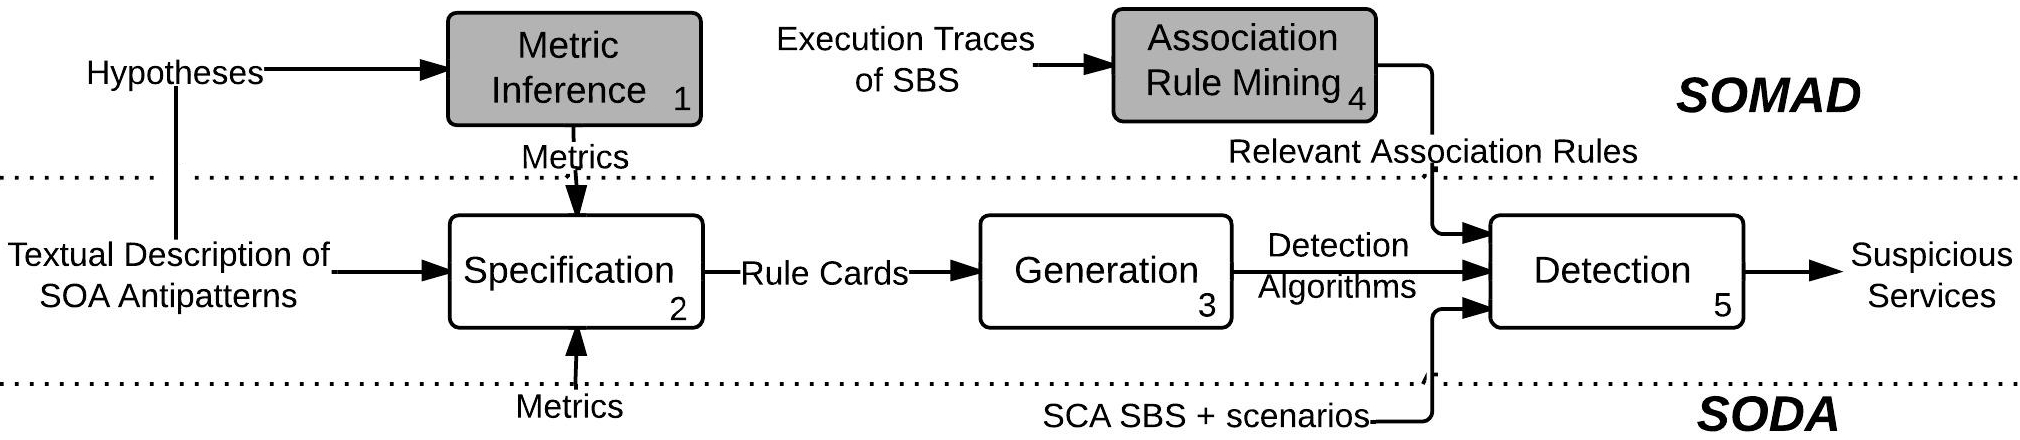
\includegraphics[scale=0.25]{media/SODA.png}%
\end{minipage}}
\caption{\label{fig:The-SODA-approach}SODA and SOMAD approaches: Grey boxes depict new steps in SOMAD w.r.t. to SODA (white boxes).}
\end{figure*}

\emph{Specification of SOA Antipatterns}: Relevant properties of SOA antipatterns are identified, which essentially correspond to metrics such as cohesion, coupling, number of methods, response time and availability. These properties compose to a base vocabulary of a DSL: a rule-based language is used whereby each rule expresses tendencies in metric values. An antipattern is described by a set of rules combined into a \textit{rule card}.

\vspace{0.12cm}

\emph{Generation of Detection Algorithms}: Automatic generation of detection algorithms is performed by visiting models of rule cards specified during the previous step. The process is straightforward and ends up with a set of directly executable algorithms.
%The generation process relies on Java code templates that correspond to the detection algorithms. .

\vspace{0.12cm}

\emph{Detection of SOA Antipatterns}: The detection algorithms generated in the previous step are applied on the SBS of interest. This step allows the automatic detection of SOA antipatterns using a set of predefined scenarios to invoke service interfaces. At the end, services from the SBS suspected of being involved in an antipattern are identified.

\vspace{0.15cm}

Although efficient and precise, SODA is an intrusive approach because it requires a set of valid scenarios concretely invoking the interface methods of SBSs and its dynamic analysis involves SCA properties. 

%
%\textcolor{blue}{\emph{Step 1. Specify SOA antipatterns:} This step lies in identifying properties in SBSs relevant to SOA antipatterns. 
%To achieve the specification we perform a thorough domain analysis of SOA antipatterns by analyzing their definitions and specification in the literature to identify relevant properties. These properties are used as a base vocabulary (Cohesion, Coupling, ...) to a DSL, in the form of a rule-based language for specifying antipatterns.}
%
%\textcolor{blue}{\emph{Step 2. Generate detection algorithms: }In this step, detection algorithms are generated automatically from the specifications defined in the previous step. Using the previous specification and our DSL; we implemented the generations as a set of visitors on models of the antipatterns rule card (rule cards are combination of rules). These algorithms are directly executable.} 
%
%\textcolor{blue}{\emph{Step 3. Detection: }Detect automatically SOA antipatterns: The third step consists of applying, on the SBSs of interest, the detection algorithms generated in \emph{Step 2} to detect SOA antipatterns.}
